\documentclass[22pt]{beamer}
% \documentclass[handout]{beamer}
% add theme and color theme https://www.overleaf.com/learn/latex/Beamer#Reference_guide
\setbeamertemplate{navigation symbols}{} % hides navigation buttons
\setbeamertemplate{footline}[frame number]
\usepackage[utf8]{inputenc}
\usepackage{minted}
\usepackage{graphicx}
\usepackage{tikz}
\usetikzlibrary{shadows}
\usepackage[absolute,overlay]{textpos}
\usepackage{comment}
\usepackage{color}
\usepackage{xcolor}
\usepackage{hyperref}
\usepackage{enumitem}
\usepackage{caption}
\setlist[itemize]{label=\textbullet, labelsep=1em, leftmargin=2em}
\usepackage{caption}
\usepackage[normalem]{ulem}
\usepackage{tcolorbox}  % For creating colored boxes
\usepackage[absolute,overlay]{textpos}

% Configure the hyperref package
\hypersetup{
    colorlinks=true,         % Color the link text
    linkcolor=blue,          % Color for internal links (e.g., \ref, \pageref)
    filecolor=blue,          % Color for file links
    citecolor=blue,          % Color for citation links
    urlcolor=blue            % Color for URLs (e.g., \href, \url)
}

% Redefine \href to include underlining
\renewcommand{\href}[2]{\textcolor{blue}{\uline{#2}}}

\newcommand{\code}[1]{\colorbox{gray!10}{\texttt{#1}}}
\newcommand{\desclabel}[1]{\textcolor{cyan}{#1}}
\newcommand{\codeTour}{
    \begin{textblock*}{1.3cm}(11cm,0.5cm) % {block width}(xcoord, ycoord)
    
\includegraphics[width=1.3cm]{Bilder/CodeTour.png}
    \end{textblock*}
}
\newcommand{\terminal}{
    \begin{textblock*}{1.3cm}(11cm,0.5cm) % {block width}(xcoord, ycoord)
    
\includegraphics[width=1.3cm]{Bilder/terminal2.png}
    \end{textblock*}
}
\newcommand{\codeTerminal}{
    \begin{textblock*}{1.3cm}(11cm,0.5cm) % {block width}(xcoord, ycoord)
        
\includegraphics[width=1.3cm]{Bilder/CodeTour.png}
    \end{textblock*}
    \begin{textblock*}{1.3cm}(9.5cm,0.5cm) % {block width}(xcoord, ycoord)
        
\includegraphics[width=1.3cm]{Bilder/terminal2.png}
    \end{textblock*}
}
\newcommand{\todo}[1]{\begingroup\sethlcolor{red}\textcolor{white}{\hl{#1}}\endgroup}

\usemintedstyle{tango}
\pagenumbering{roman}

\title{Docker something}
\author{Julia Winkler}
\date{19.06.2024}

\begin{document}

%% TODO: layout element, dass kennzeichnet, wann man ins terminal wechselt vgl. "Vorlesung" bei EAE
%% TODO: how to make one list item without overhead -> macro?
%% einheitliche Sprache
%% teerminal Bild gleiches Format

\begin{frame}[plain]
    \vfill
    \begin{center}
        
\includegraphics[width=1\textwidth]{Bilder/docker-how.png}
    \end{center}
    \vfill
\end{frame}

\begin{frame}[t]
    \frametitle{Disclaimer}
    \begin{itemize}
        \item bei weitem nicht alles zum Thema Docker
        \item nur Allgemeine Grundlage
    \end{itemize}

    \begin{textblock*}{4.5cm}(1.5cm,4cm) % {block width}(xcoord, ycoord)
        \begin{figure}
            
\includegraphics[width=1.5cm]{Bilder/terminal2.png}
            \captionsetup{justification=centering}
            \caption*{Befehle im Terminal ausführen\\ Ordner \code{examples}, wenn nichts da steht}
        \end{figure}

    \end{textblock*}

    \begin{textblock*}{4.5cm}(7.2cm,4cm) % {block width}(xcoord, ycoord)
        \begin{figure}
            
\includegraphics[width=1.5cm]{Bilder/CodeTour.png}
            \centering
            \captionsetup{justification=centering}
            \caption*{CodeTour (VSCode Plugin)\\Code im Repo}
        \end{figure}
    \end{textblock*}

\end{frame}

\begin{frame}[plain]
    \frametitle{Gliederung}
    \tableofcontents
\end{frame}

\section{Einführung}
\begin{frame}[t]
    \frametitle{Das Wichtigste zuerst}\pause
    \only<2>{\begin{figure}[h]
        \centering
        
\includegraphics[width=0.8\textwidth]{Bilder/mobydocker.jpg}
    \end{figure}
    }
    \only<3>{\begin{figure}[h]
        \centering
        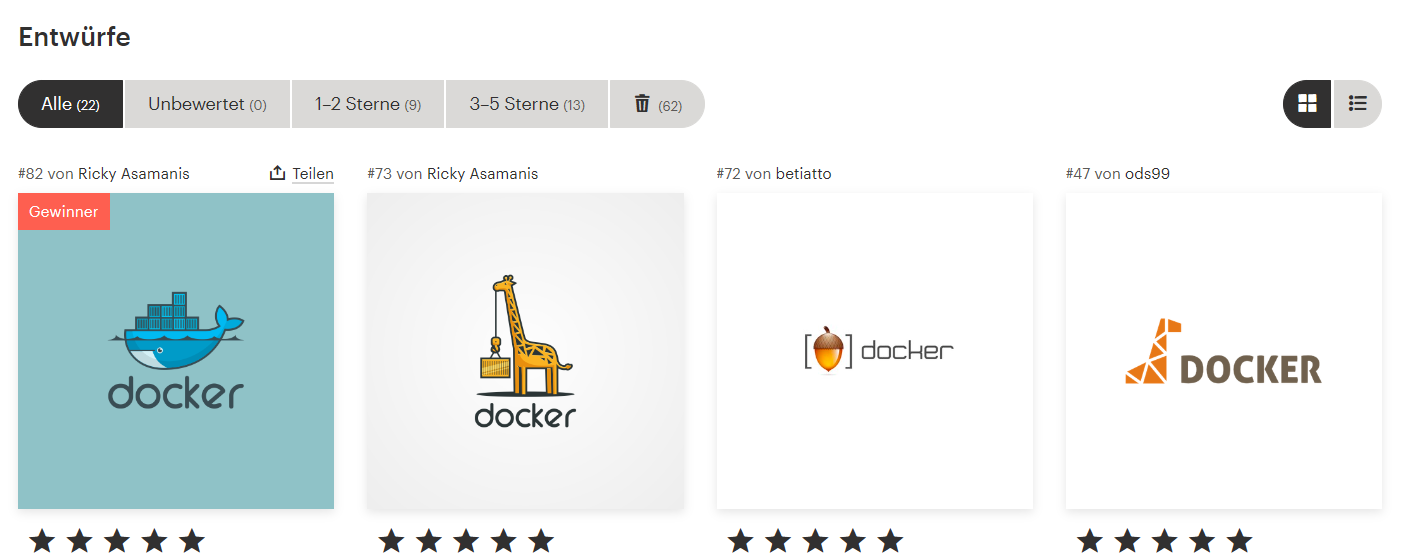
\includegraphics[width=0.95\textwidth]{Bilder/wettbewerb.png}
        \caption*{Wettbewerb zum Icon für Docker}
    \end{figure}
    }
\end{frame}

\begin{frame}[t]
    \frametitle{Wiso, Weshalb, Warum?}
    \begin{center}
        
\includegraphics[width=0.8\textwidth]{Bilder/docker-why.png}
    \end{center}\pause
    \begin{center}
        "a sandboxed process on your machine that is isolated from all other processes on the host machine"
    \end{center}\pause
    \begin{center}
        "faster onboarding and testing while also simplifying the deployment of services"
    \end{center}\pause
    \begin{center}
        "Nachdem ich im letzten Talk öffentlichkeitswirksam meine Docker-Compose Config versemmelt habe, forder ich hiermit für nächstes Semester eine Einführung in Docker, damit mir, das nicht nochmal passiert" - Tim Hegemann
    \end{center}
\end{frame}

\begin{frame}
    \frametitle{Wiso, Weshalb, Warum?}
    \begin{center}
        
\includegraphics[height=0.8\textheight]{Bilder/Meme.png}
    \end{center}
\end{frame}

\begin{frame}[t]
    \frametitle{Was ist Docker?}
    \begin{block}{Docker}
        freie Software zur Isolierung von Anwendungen\newline
        Containervirtualisierung\newline
        "light weight" Virtual Maschine\newline
    \end{block}
    \begin{figure}[h]
        \centering
        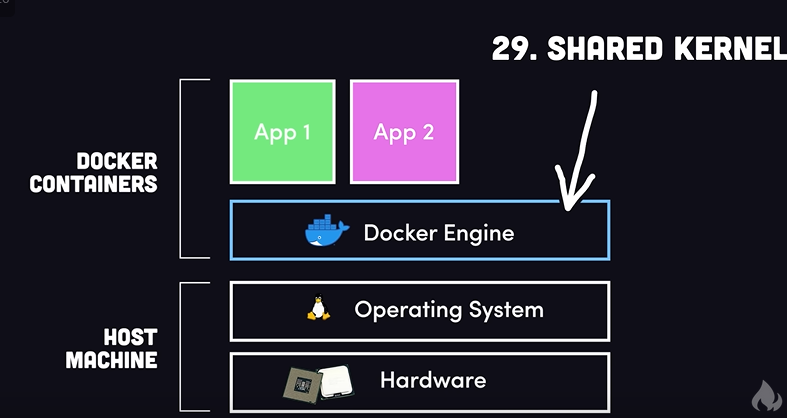
\includegraphics[width=0.9\textwidth]{Bilder/Docker Concept.png}
    \end{figure}
\end{frame}


\begin{frame}[t]
    \frametitle{Wichtige Begriffe}
    \begin{block}{Dockerfile}
        Anleitung, um ein Image zu erstellen
    \end{block}
    \begin{block}{Image}
        Blaupausen, um einen Container zu erstellen
    \end{block}
    \begin{block}{Container}
        Umgebung in der die tatsächliche Anwendung läuft
    \end{block} \pause
    \begin{block}{Registry}
        z.B. Docker Hub, EAC....
        Ort an dem viele verschindene Images gespeichert und geteilt werden können
    \end{block}
    \begin{block}{Docker Compose}
        Orchestrierungstool für Dockerfile\newline
        Wrapper für einen oder mehrere Container
    \end{block}
    %%\begin{block}{Docker Desktop}
    %%    - UI für alles was man in der CLI machen kann (?) %% TODO: 
    %%\end{block}
\end{frame}

\begin{frame}[c]
    \frametitle{Zusammenhang der Docker Komponenten}
        \includegraphics<1>[width=1\textwidth]{Bilder/Docker-Ablauf.png}
        \includegraphics<2>[width=1\textwidth]{Bilder/dockercommand.png}
\end{frame}

\begin{frame}[c]
    \frametitle{Wie kreige ich dieses "Docker"?}
    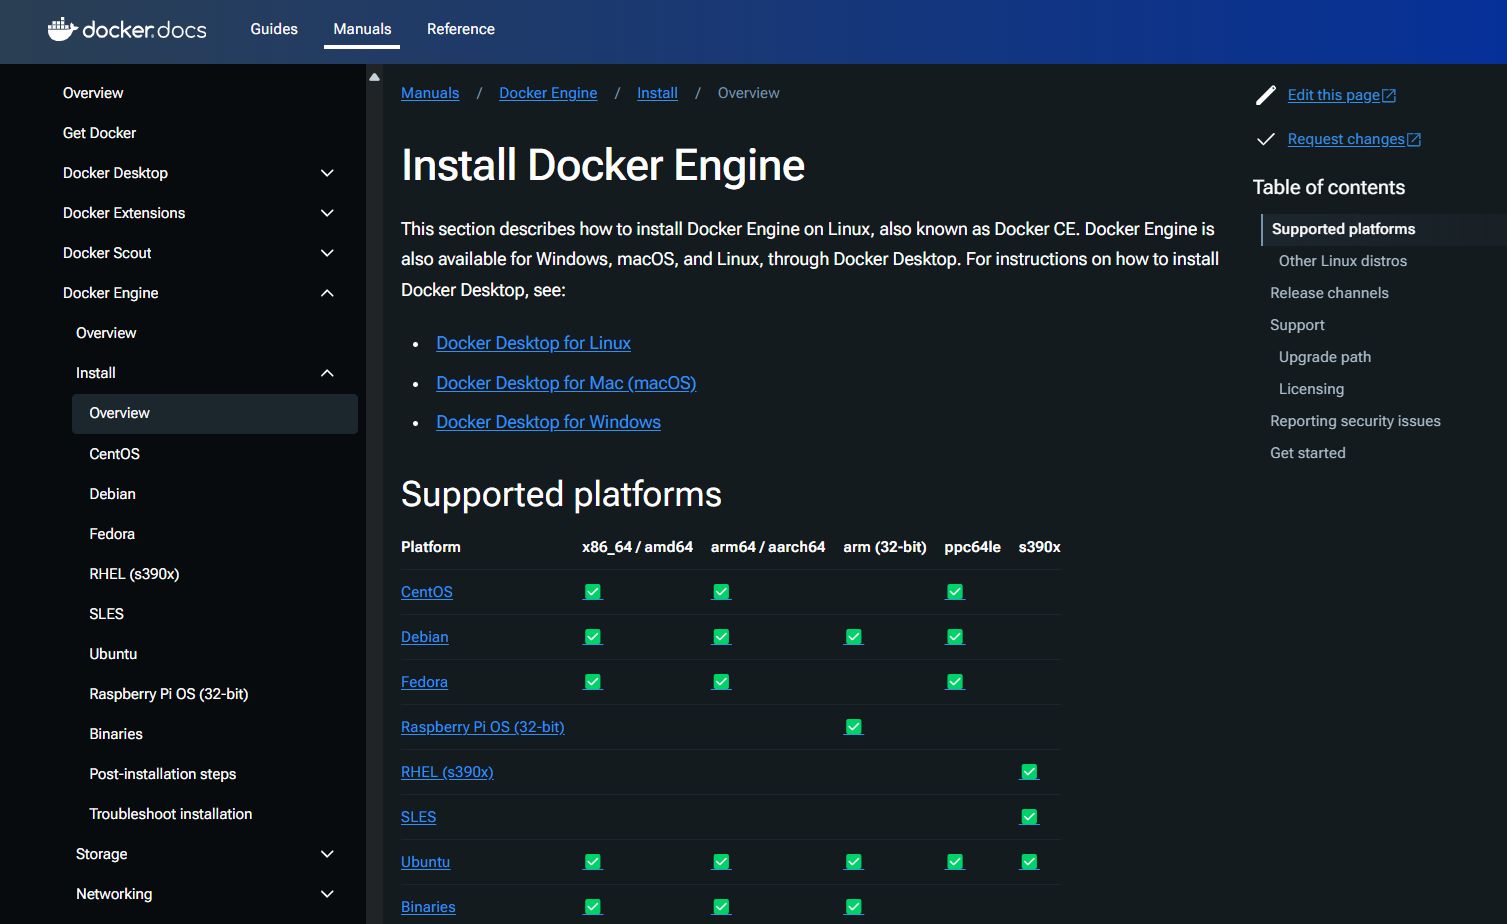
\includegraphics[width=0.9\textwidth]{Bilder/Installation.png}

    \href{https://docs.docker.com/engine/install}{Doku}
\end{frame}

\begin{frame}[fragile,t]
    \frametitle{Hello World}
    \terminal
\begin{minted}{bash}
> docker -v
> docker --help
> docker run hello-world
\end{minted}
\end{frame}

\section{Dockerfile}
\begin{frame}[c]
    \frametitle{Zusammenhang der Docker Komponenten}
    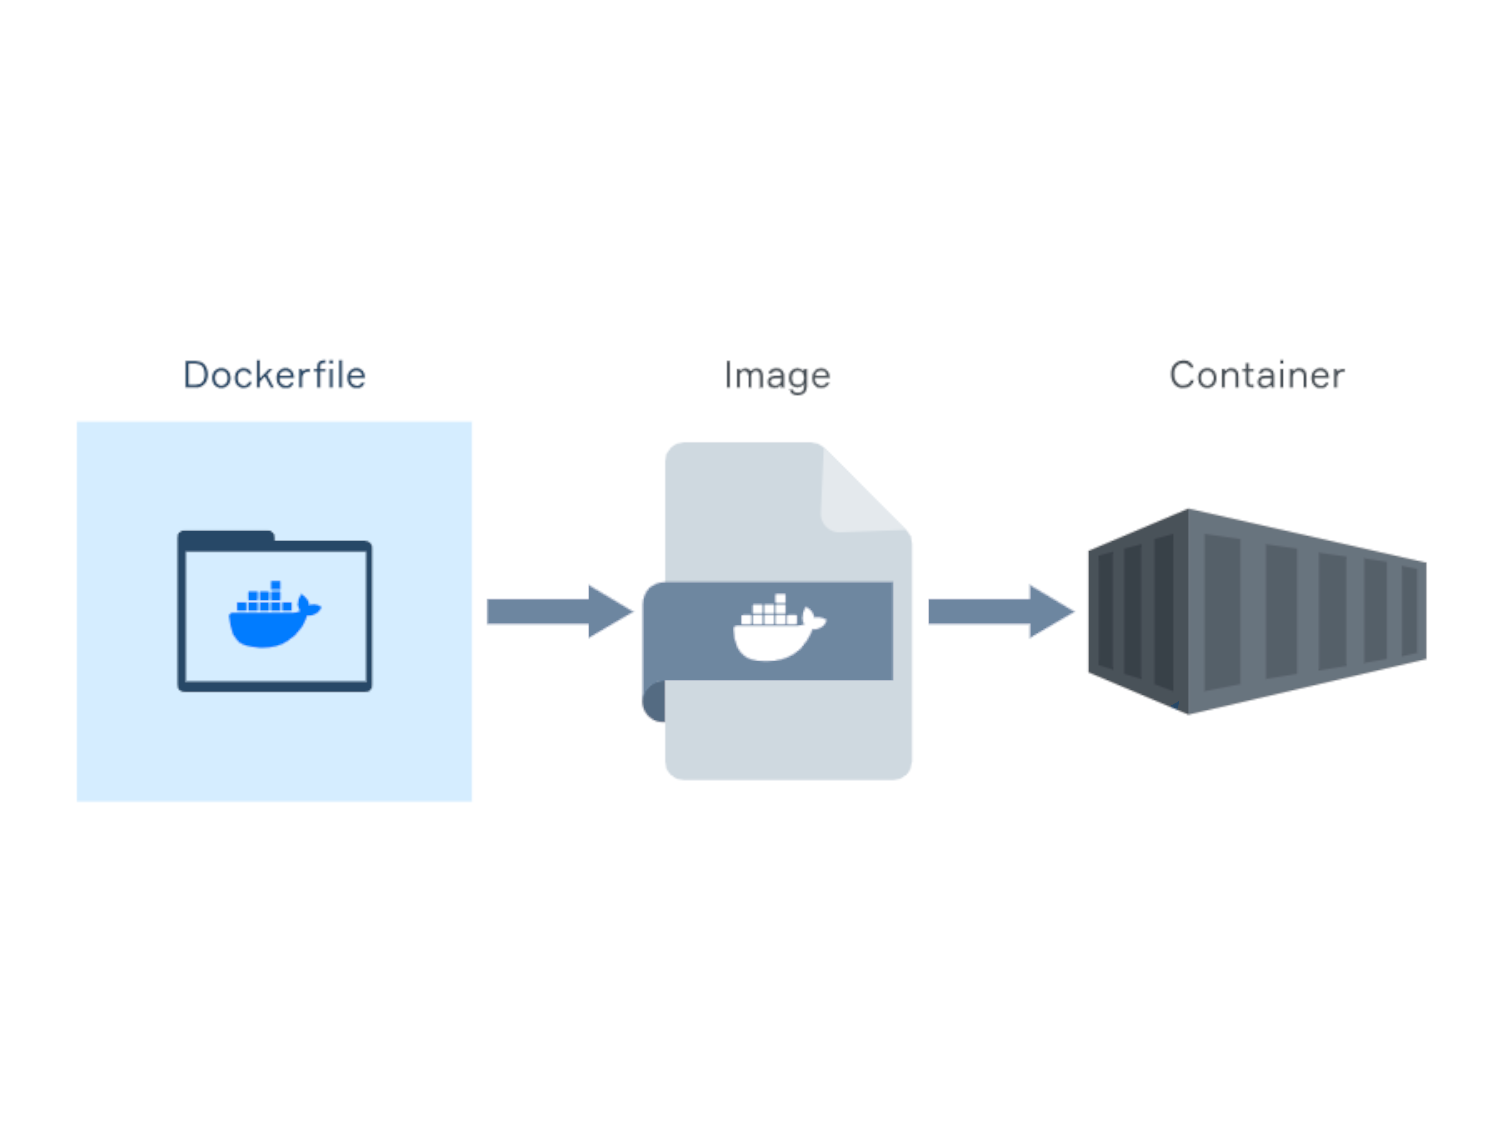
\includegraphics[width=1\textwidth]{Bilder/Docker-Ablauf_file.png}
\end{frame}

\begin{frame}[fragile]
    \frametitle{Dockerfile}
    \begin{itemize}
        \item Anleitung um ein Image zu erstellen
        %% Mit einem Dockerfile kann man den Inhalt des Containers configurieren
        \item hießt standardmäßig 'Dockerfile'
        \item \code{INSTRUCTION ARG1 ...}
    \end{itemize}
    \only<1>{\codeTour}

    ein beispielhaftes \code{Dockerfile}: 
    \inputminted[fontsize=\footnotesize, frame=lines]{Dockerfile}{../examples/Dockerfile}\medskip 
    \pause
    Weitere Informationen und Instruction
    \href{https://docs.docker.com/reference/dockerfile/#overview}{https://docs.docker.com/reference/dockerfile/}

\end{frame}

\section{Einfache Container}
%% Überleitung: Wie kommt man jetzt vom Dockerfile zum Image
\begin{frame}[c]
    \frametitle{Zusammenhang der Docker Komponenten}
    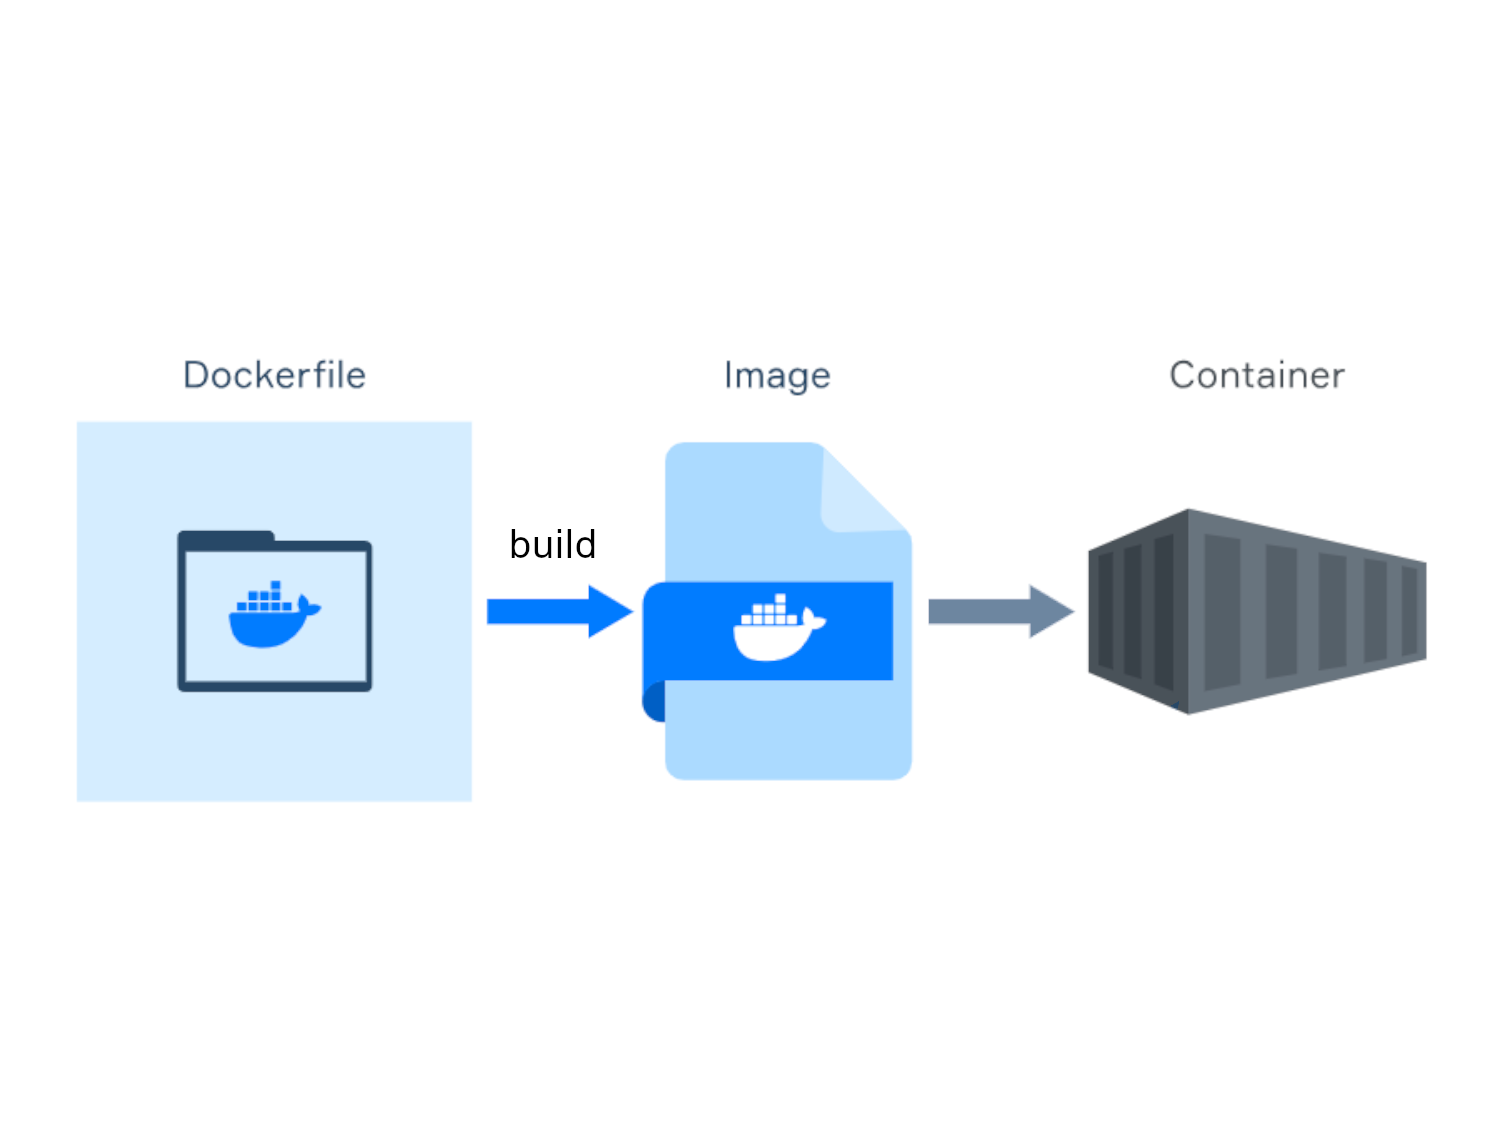
\includegraphics[width=1\textwidth]{Bilder/Docker-Ablauf_build.png}
\end{frame}

\begin{frame}[fragile]
    \frametitle{docker build Befehl}
    \code{docker build [OPTIONS] PATH | URL | -} 
    
    \-  \ Erstelle ein Image aus einem Dockerfile\vspace{5pt}
    
    \code{[OPTIONS]}
    \begin{description}[labelindent=0.5cm, style=unboxed, labelwidth=\widthof{-f, -\,-file string}, leftmargin=!]
        \item[\desclabel{-t, -\,-tag stringArray}] Name und optionaler Tag für das Image (format: "name:tag")
        \item[\desclabel{-f, -\,-file string}] Name des Dockerfile
        \item[...] 
    \end{description}
    
    \code{PATH} Pfad zum Build Kontext (Ordner), meistens \code{.}
    \pause
    Beispiele
    \begin{minted}[fontsize=\small]{bash}
    docker build . # 'Dockerfile' im aktuellen Ordner
    docker build -t myimage:v1 . 
    docker build -f Dockerfile.cmd . 
    docker build FastAPI
    \end{minted}
    \medskip

    {\small weitere Optionen mit \code{docker buildx build}}
\end{frame}

\begin{frame}[fragile, b]
    \frametitle{RUN}
    \terminal
    \begin{columns}
        \begin{column}{0.5\textwidth}
            \inputminted[fontsize=\scriptsize, frame=lines]{dockerfile}{../examples/Dockerfile.multi}
        \end{column}
        \begin{column}{0.5\textwidth}
            \inputminted[fontsize=\scriptsize, frame=lines]{dockerfile}{../examples/Dockerfile.single}
        \end{column}
    \end{columns}
    \medskip\pause
\begin{minted}{bash}
> docker build -t example:multi -f Dockerfile.multi .
> docker build -t example:single -f Dockerfile.single .
# Vergleicht die Build-time

# Vergleicht die Größe - Wie?
> docker images # Entstandene Images anschauen

\end{minted}
\end{frame}

\begin{frame}[fragile]
    \frametitle{RUN}
    \begin{columns}
        \begin{column}{0.5\textwidth}
            \inputminted[fontsize=\scriptsize, frame=lines]{dockerfile}{../examples/Dockerfile.multi}
        \end{column}
        \begin{column}{0.5\textwidth}
            \inputminted[fontsize=\scriptsize, frame=lines]{dockerfile}{../examples/Dockerfile.single}
        \end{column}
    \end{columns}
    \medskip
    \begin{itemize}
        \item<1-> pro \code{RUN} baut Docker einen Layer
        \item<2-> mehr Layer vergrößern das Image
        \item<2-> Layer werden gecached und nach Möglichkeit wiederverwendet
        \item<3-> verbinden von \code{RUN} instructions verbessert built time und Image Größe
    \end{itemize}
\end{frame}

\begin{frame}[fragile, t]
    \frametitle{CMD vs. ENTRYPOINT}
    %% TODO: pre build images
    %% Comment: Experementiert das gerne etwas mit rum, zwei Entry Points, CMD und Entrypoint gemischt
    \terminal
    \begin{columns}[t]
        \begin{column}{0.5\textwidth}
            \inputminted[fontsize=\scriptsize, frame=lines]{dockerfile}{../examples/Dockerfile.cmd}
        \end{column}
        \begin{column}{0.5\textwidth}  %%<--- here
            \inputminted[fontsize=\scriptsize, frame=lines]{dockerfile}{../examples/Dockerfile.entry}
        \end{column}
    \end{columns}
    \medskip
\begin{minted}{bash}
> docker build -t example:cmd -f Dockerfile.cmd .
> docker build -t example:entry -f Dockerfile.entry .
\end{minted} 
\pause\medskip
%% demo docker run example:cmd hello
\begin{minted}{bash}
> docker run example:cmd
> docker run example:cmd echo hello
> docker run example:entry hello        
\end{minted}
\end{frame}

\begin{frame}[fragile, t]
    \frametitle{CMD vs. ENTRYPOINT}
    \begin{columns}[t]
        \begin{column}{0.5\textwidth}
            \inputminted[fontsize=\scriptsize, frame=lines]{dockerfile}{../examples/Dockerfile.cmd}
        \end{column}
        \begin{column}{0.5\textwidth} 
            \inputminted[fontsize=\scriptsize, frame=lines]{dockerfile}{../examples/Dockerfile.entry}
        \end{column}
    \end{columns}
    \medskip
    \begin{itemize}
        \item beide definieren den, was nach Container start ausgeführt wird
        \item \code{CMD} kann überschrieben werden
        \item \code{ENTRYPOINT} bestimmt den Befehl(Executable), neue Parameter werden angehangen
    \end{itemize}
\end{frame}


\begin{frame}[c]
    \frametitle{Zusammenhang der Docker Komponenten}
    %% Zusammenhang Image haben wir jetzt, wie wird aus dem Image ein Conatiner
    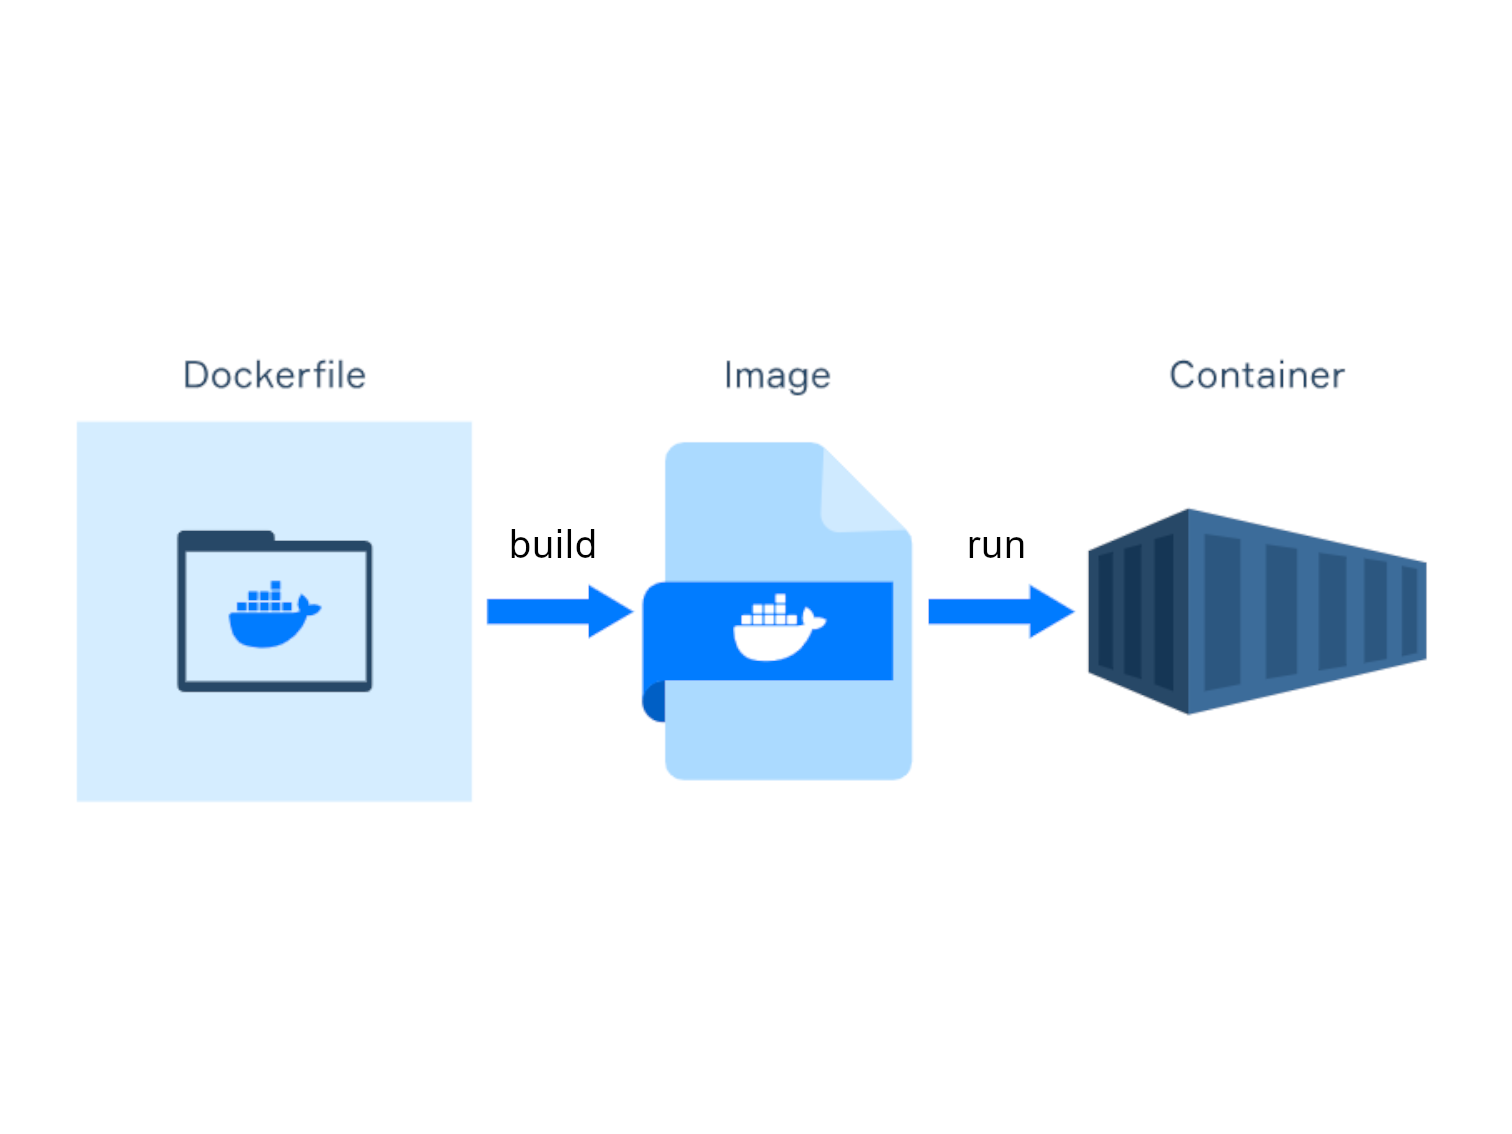
\includegraphics[width=1\textwidth]{Bilder/Docker-Ablauf_full.png}
\end{frame}

\begin{frame}
    \frametitle{docker run Befehl}
    \code{docker run [OPTIONS] IMAGE [COMMAND] [ARG...]}

    \-  \ Erstelle und starte einen Container von einem Image\vspace{5pt}

    \code{[OPTIONS]}
    \begin{description}[labelindent=0.5cm, style=unboxed, labelwidth=\widthof{-\,-mount mountm}, leftmargin=!]
        \item[\desclabel{-d}] Container vom Terminal lösen
        \item[\desclabel{-\,-name}] Container bennen
        \item[\desclabel{-it}] Interaktives Terminal im Container öffnen
        \item[\desclabel{-e}] Umgebungsvariablen setzen
        \item[\desclabel{-p [host]:[port]}] Port(s) veröffentlichen
        \item[\desclabel{-P}] Alle Ports veröffentlichen
        \item[\desclabel{-\,-rm}] Container nach Beenden entfernen
    \item[\desclabel{-\,-mount mount}] Dateisystem and den Container mounten
        \item[\desclabel{-v, -\,-volume list}] Bind mount ein Volume
        \item[...] 
    \end{description}
    \code{IMAGE} Referenz zum Image (Tag oder Id/Hash)
\end{frame}

\begin{frame}[plain]
    \frametitle{Python / FastAPI}
    \begin{textblock*}{\paperwidth}(1cm, 2cm) % {block width}(xcoord, ycoord)
        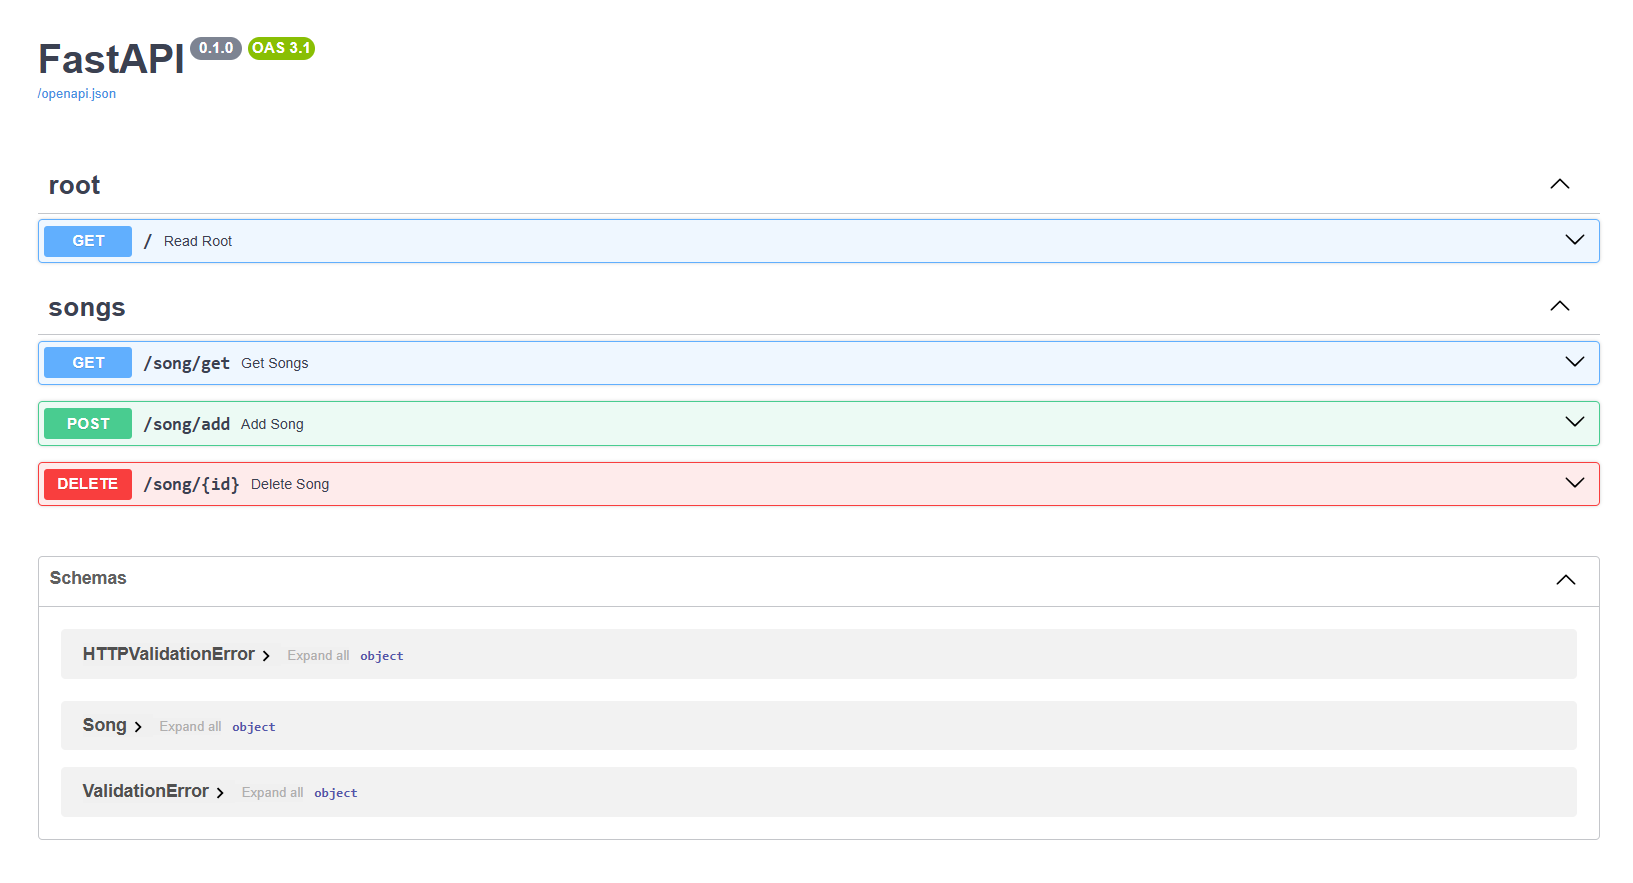
\includegraphics[width=0.85\paperwidth]{Bilder/Fastapi.png}
        \end{textblock*}
\end{frame}


\subsection{Beispiel: Python (FastAPI) \& Basic Befehle}
\begin{frame}[fragile]
    \codeTour
    \frametitle{Python FastAPI im Conatiner}

    \inputminted[fontsize=\footnotesize, frame=lines]{dockerfile}{../examples/FastAPI/Dockerfile}
\end{frame}

\begin{frame}[fragile]
    \frametitle{Python FastAPI im Conatiner}
    \terminal
\begin{minted}{bash}
> cd examples/FastAPI
> docker build -t fastapiapp:v1 .
> docker run --name backend -p 8000:80 fastapiapp:v1
# Open http://localhost:8000/docs
> docker start backend
> docker stop backend
> docker rm backend
> docker run -d --name --rm backend \
    -p 8000:80 fastapiapp:v1
> docker exec -it backend bash
# 'exit' um den Container zu verlassen
\end{minted}
    %% stoppen
    %% Überleitung: beim zweiten start Songs hinzugügen, 
    %% nach dem remove neuen Container, der hat die Songs nicht
\end{frame}

\begin{frame}[fragile]
    \frametitle{docker exec Befehl}
    \code{docker exec [OPTIONS] CONTAINER COMMAND [ARG...]}

    \-  \ Befehl in einem laufenden Container ausführen\vspace{5pt}

    \code{[OPTIONS]}
    \begin{description}[labelindent=0.5cm, style=unboxed, labelwidth=\widthof{bla}, leftmargin=!]
        \item[\desclabel{-d}] im Hintergund ausführen
        \item[\desclabel{-e}] env Variablen setzen
        \item[\desclabel{-it}] Interaktives Terminal öffnen
        \item[\desclabel{-w, -\,-workdir string}] Aktuelles Verzeichnis im Container ändern
        \item[...] 
    \end{description}

    Beispiele:
\begin{minted}[fontsize=\small]{bash}
docker exec -it backend bash # Interaktives Terminal öffnen
docker exec -d backend touch /code/README.md
docker exec -e VAR_A=1 -e VAR_B=2 backend env
\end{minted}
    
\end{frame}

\begin{frame}
    \frametitle{docker container control Befehl}

    \code{docker create [OPTIONS] IMAGE [COMMAND] [ARG...]}\\
    \-  \ Erstelle einen Container ohne ihn zustarten \medskip

    \code{docker start [OPTIONS] CONTAINER [CONTAINER...]}\\
    \-  \ Starte einen oder mehrere exitierende Container \medskip

    \code{docker stop [OPTIONS] CONTAINER [CONTAINER...]}\\
    \-  \ Stoppe einen oder mehrere laufende Container (SIGTERM) \medskip

    \code{docker pause CONTAINER [CONTAINER...]}\\
    \-  \ Stoppe alle Prozesse innerhalb eines oder mehrerer Conatiner \medskip

    \code{docker kill [OPTIONS] CONTAINER [CONTAINER...]}\\
    \-  \ Stoppe einen oder mehrere laufende Container (SIGKILL) \medskip
    
\end{frame}

\begin{frame}
    \frametitle{docker remove Befehle}
    \code{docker rm [OPTIONS] CONTAINER [CONTAINER...]}

    \- \ Entferne einen oder mehrere Container\vspace{5pt}

    \code{[OPTIONS]}
    \begin{description}[labelindent=0.5cm, style=unboxed, labelwidth=\widthof{-v, -\,-volumess}, leftmargin=!]
        \item[\desclabel{-f, -\,-force}] Erzwinge das Entfernen
        \item[\desclabel{-v, -\,-volumes}] Verbundene anonyme Mounts auch entfernen
    \end{description}\medskip\medskip
    \code{docker rmi [OPTIONS] IMAGE [IMAGE...]}

    \- \ Entferne ein oder mehrere Images\vspace{5pt}

    \code{[OPTIONS]}
    \begin{description}[labelindent=0.5cm, style=unboxed, labelwidth=\widthof{-\,-no-prunes}, leftmargin=!]
        \item[\desclabel{-f, -\,-force}] Erzwinge das Entfernen
        \item[\desclabel{-\,-no-prune}] Do not delete untagged parents
    \end{description}
\end{frame}

\begin{frame}[fragile, t]
    \frametitle{Wo ist mein Song?}
    Problem reproduzieren:
\begin{minted}[fontsize=\footnotesize]{bash}
> cd examples/FastAPI
> docker build -t fastapiapp:v1 .
> docker run -d --name backend -p 8000:80 --rm fastapiapp:v1
# Öffne http://localhost:8000/docs + add_song() ausführen
> docker stop backend # Container automatisch gelöscht
> docker run -d --name backend -p 8000:80 --rm fastapiapp:v1
# get_songs() ausführen -> Song fehlt :/
\end{minted}
\pause\medskip
    \begin{itemize}
        \item der Song ist im Container gespeichert, nicht im Image
        \item \code{-\,-rm} löscht den Container nach Beendigung
    \end{itemize}
    \vspace{0.6cm}
    Wie bekomme ich den Song permantent gespeichert?
\end{frame}

\begin{frame}[fragile]
    \frametitle{Python FastAPI im Conatiner}
    \only<2->{\terminal}
    \begin{itemize}
        \item<1-> Option 1: json anpassen, Image neu erstellen
        \item<2-> Option 2: Änderungen commiten
        \item<3-> Option 3: Volumes und Mounts verwenden
    \end{itemize}\pause
    \medskip
\begin{minted}{bash}
> docker commit backend fastapiapp:v2
> docker run -d --name backend2 --rm \
    -p 8080:80 fastapiapp:v2
# Öffne localhost:8080/docs -> get_songs() hat neue Songs

> docker run -d -\,-name backend ,-rm \
    -p 8000:80 fastapiapp:v1
# Öffne localhost:8000/docs -> get_songs() hat keine
\end{minted}
\end{frame}

\subsection{Volumes und Mounts}
\begin{frame}[t]
    \frametitle{Volumes und Mounts}
    \begin{itemize}
        \item Docker Container sind stateless
        \item beide verbinden Speicher/Verzeichnisse vom der Host Maschine zu Speicher im Container
    \end{itemize} \pause
    \begin{block}{Volume}
        \begin{itemize}
            \item gemanaged von Docker (standardmäßig: \code{var/lib/docker/volumes/VOLUMENAME})
            \item vergrößern nicht die Container
            \item vereinfachen und ermöglichen das teilen von Daten zwischen Containern
        \end{itemize}
    \end{block} \pause
    \begin{block}{Mount}
        \begin{itemize}
            \item Datei/Ordner vom Host an den Container anbinden
            \item abhängig von der Host Maschine
        \end{itemize}
    \end{block}
\end{frame}

\begin{frame}[fragile]
    \frametitle{Python FastAPI im Conatiner mit Volume}
    \terminal
    \begin{itemize}
        \item Option 1: json anpassen, Image neu erstellen
        \item Option 2: changes commiten
        \item Option 3: Volume, wenn man die json changes behalten möchte, aber den container per se nicht
    \end{itemize}
\vspace{0.8cm}
\begin{minted}{bash}
# Note: be aware of the working directory of your app
# in this case code 'WORKDIR /code'
> docker run -d --rm --name backend \
    -v ${PWD}/app/songs.json:/code/app/songs.json \
    -p 8000:80 fastapiapp:v1 
\end{minted}
            
\end{frame}

\begin{frame}[t]
    \begin{textblock*}{\paperwidth}(0.7cm,0.5cm) % {block width}(xcoord, ycoord)
        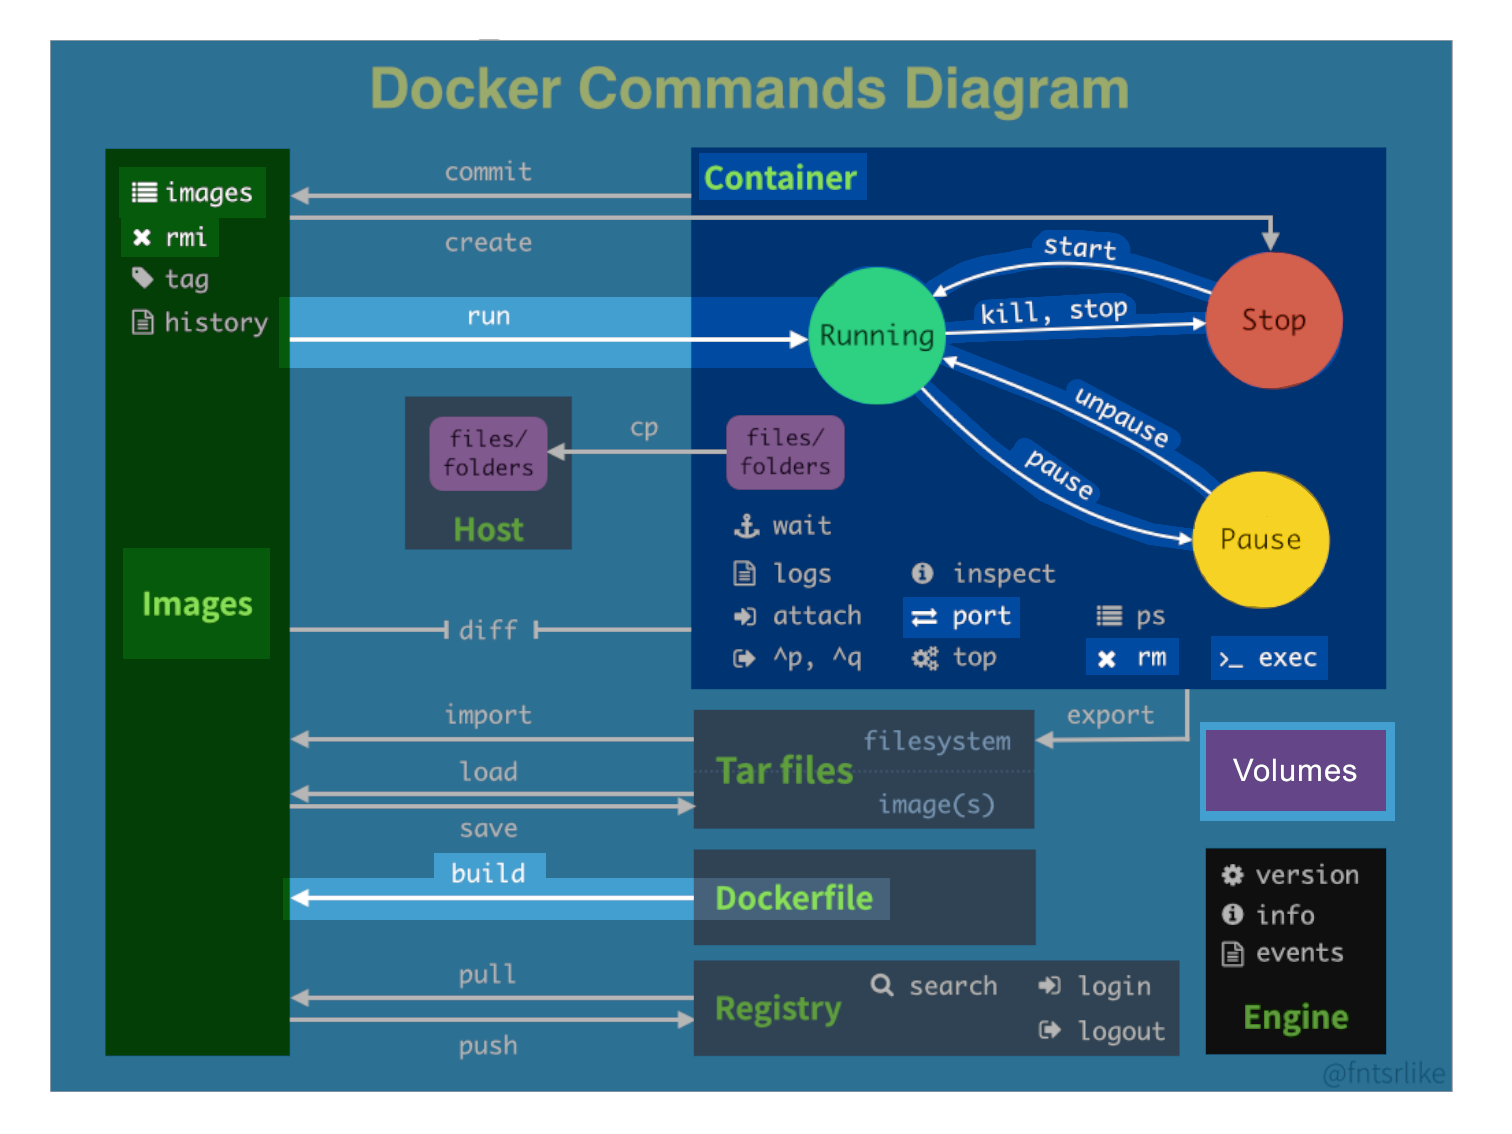
\includegraphics[width=0.9\paperwidth]{Bilder/Commands_Zf.png}
    \end{textblock*}
\end{frame}  

\subsection{React}
%% Überletung jetzt wollen wir natürlich auch noch eine Oberfläche

    
\begin{frame}[c]
    \frametitle{React}
    \begin{textblock*}{\paperwidth}(1cm, 2cm) % {block width}(xcoord, ycoord)
        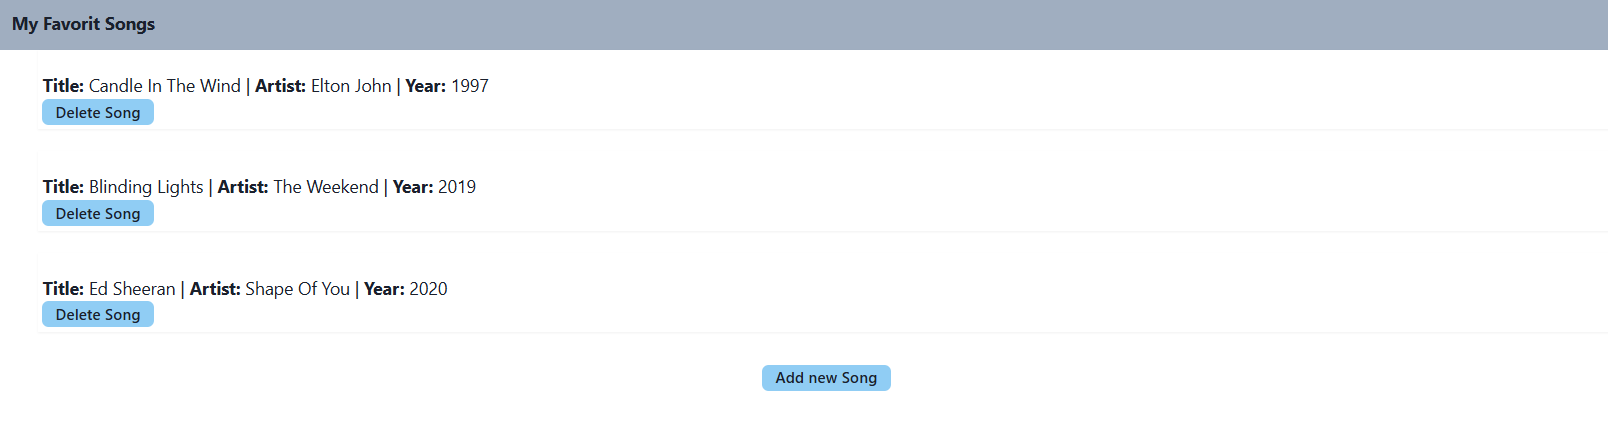
\includegraphics[width=0.85\paperwidth]{Bilder/Webseite.png}
    \end{textblock*}
\end{frame}

\begin{frame}[fragile]
    \frametitle{React - Dockerfile}
    \inputminted[fontsize=\footnotesize, frame=lines]{dockerfile}{../examples/React/Dockerfile}
\end{frame}

\begin{frame}[fragile]
    \frametitle{React im Container}
    \terminal
%% node aus container app lokal
\begin{minted}{bash}
> cd examples/React
> docker build -t reactapp:dev .
> docker run -it --rm --name frontenddev \
    -v ${PWD}:/app -v /app/node_modules \
    -e CHOKIDAR_USEPOLLING=true \ # enable hot-reloading
    -p 3000:3000  reactapp:dev
# Öffne localhost:3000

\end{minted}
\footnotesize (Der Container \code{backend} sollte laufen, damit die Webseite richtig funktioniert)
\end{frame}

\subsection{Multistage Builds}
\begin{frame}[t]
    \frametitle{Multistage builds}
    Idee: Image aufeinanderaufbauende Teile teilen, zwischen den Teilen nur die nötigen Dinge kopieren

    z.B. Stage 1: App compile, Stage 2: Compilierte App ausführen (kein Build context) 
    \pause
    Vorteile
    \begin{itemize}
        \item Smaller image size
        \item faster build times
        \item improved security (only runtime artifacts and dependencies)
        \item code isolation and reusability
        \item Easier debugging and troubleshooting
    \end{itemize} 
\end{frame}

\begin{frame}[fragile]
    \frametitle{React - Multistage}
    \inputminted[fontsize=\footnotesize, frame=lines]{dockerfile}{../examples/React/Dockerfile.prod}
\end{frame}

\begin{frame}[fragile]
    \frametitle{React - Multistage}
    \terminal
\begin{minted}{bash}
> docker build -f Dockerfile.prod -t reactapp:prod .
> docker run -it --rm --name frontend \
    -p 1337:80 reactapp:prod
# Öffne localhost:1337
\end{minted}
\vspace{8pt}
Vergleiche die Größe der Images:\pause

frontenddev: 832 MB

frontend: 50.9 MB

\end{frame}

\begin{frame}[t]
    \frametitle{Dockerfile Best Practices}
    \begin{itemize}
        \item \code{RUN} instructions mit \&\& zusammenfassen
        \item \code{COPY} sinnvoll platzieren, damit Cache best möglich genutzt werden kann
        \item \code{ADD} nur für \code{ADD} spezifische Funktionen
        \item Volumes und Mounts für persistententen Speicher nutzen
        \item Multistage builds verwenden
    \end{itemize} 
    \only<2>{
    \begin{figure}[h]
        \centering
        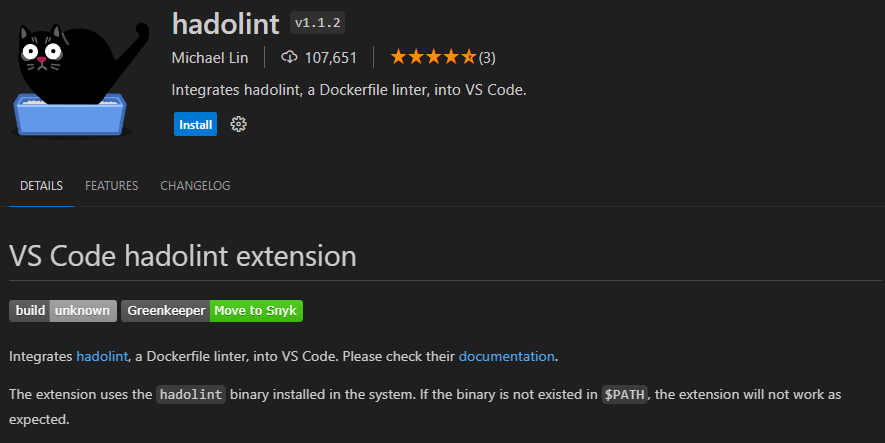
\includegraphics[width=0.6\textwidth]{Bilder/Hadolint.png}
        \caption*{Plugin für die Arbeit mit Docker}
    \end{figure}
    }
\end{frame}

\begin{frame}[fragile]
    \frametitle{Weiteres zu docker}
    \code{.dockerignore}
    \begin{itemize}
        \item vgl. .gitignore für Docker
        \item bestimmte Dateien/Ordern ausschließen
        \item geringere Image Größe
        \item kein Cache invalidation
    \end{itemize}
    \medskip\pause
    Docker Desktop bietet eine Benutzeroberfläche für die meinsten Befehle\\\pause
    \begin{minted}{bash}
# interaktion mit Registries
> docker push
> docker pull 
# Scan auf Sicherheitslücken
> docker scout   
\end{minted}
Weitere Befehle am Ende
\end{frame}
%% Pause alle Container stoppen, ggf kurz Docker Desktop zeigen
\section{Docker Compose}
\begin{frame}[plain]
    \begin{textblock*}{\paperwidth}(0cm,1.5cm) % {block width}(xcoord, ycoord)
        
\includegraphics[width=\paperwidth]{Bilder/1200px-Docker-compose-logo.jpg}
    \end{textblock*}
\end{frame}

\begin{frame}[t]
    \frametitle{Docker Compose}
    \begin{block}{Was?}
        Tool um Multi-Container Anwendungen einfach auszuführen\\
        eine Konfiguration, statt in meheren Terminals alle verschiedene Container laufen zu lassen
    \end{block}\pause
    \begin{block}{Warum?}
        \begin{itemize}
            \item leichter mit mehreren Container zuarbeiten
            \item gute Portabilität
            \item schnelle Anwendungsentwicklung
        \end{itemize}
    \end{block}\pause
    \begin{block}{Wie?}
        \begin{itemize}
            \item Definition von Services in \code{docker-compose.yml}
            \item ein Service entspricht einem Container
        \end{itemize}
    \end{block}
    \medskip
    \footnotesize Anmerkung: Python in \code{examples/FastAPI}, React in \code{examples/React} und Full App in \code{examples} ausführen
\end{frame}

\begin{frame}[fragile]
    \terminal
    \frametitle{Docker Compose zu Python}
    \inputminted[fontsize=\footnotesize, frame=lines]{dockerfile}{../examples/FastAPI/docker-compose.yml}
    \verb|docker compose up|
    \medskip\pause
    \begin{minted}{bash}
> docker build -t fastapiapp:v1 .
> docker run --rm --name backend \
    -v ${PWD}/app/songs.json:/code/app/songs.json \
    -p 8000:80 fastapiapp:v1
    \end{minted}
    \begin{textblock*}{1.3cm}(11cm,6.8cm) % {block width}(xcoord, ycoord)
        \huge \textcolor{red}{vs.}
    \end{textblock*}
\end{frame}

\begin{frame}[fragile]
    \frametitle{Docker Compose Webapp}
    \terminal
    \inputminted[fontsize=\footnotesize, frame=lines]{dockerfile}{../examples/React/docker-compose.prod.yml}
\begin{minted}{bash}
> docker-compose -d -f docker-compose.prod.yml \
    up
\end{minted}
\medskip

\begin{minted}{bash}
> docker build -f Dockerfile.prod -t reactapp:prod .
> docker run -it --rm -d --name frontend \
    -p 1337:80 frontend:prod
\end{minted}
\only<1>{
    \begin{textblock*}{6cm}(1cm,1.5cm) % {block width}(xcoord, ycoord)
        \begin{tcolorbox}[width=6cm, height=4.2cm, colback=white, colframe=white, sharp corners]
        \centering
        \end{tcolorbox}
    \end{textblock*}
}
\only<2>{}
\begin{textblock*}{1.3cm}(11cm,7cm) % {block width}(xcoord, ycoord)
    \huge \textcolor{red}{vs.}
\end{textblock*}
\end{frame}

\begin{frame}[fragile]
    \frametitle{Docker Compose Full App}
    \terminal
    \inputminted[fontsize=\footnotesize, frame=lines]{dockerfile}{../examples/docker-compose.yml}
\begin{minted}{bash}
> docker-compose up 
\end{minted}
\only<1>{
    \begin{textblock*}{6cm}(1.6cm,2.8cm) % {block width}(xcoord, ycoord)
        \begin{tcolorbox}[width=6cm, height=2.2cm, colback=white, colframe=white, sharp corners]
        \centering
        \end{tcolorbox}
    \end{textblock*}
    \begin{textblock*}{6cm}(1.6cm,5.5cm) % {block width}(xcoord, ycoord)
        \begin{tcolorbox}[width=9cm, height=3.1cm, colback=white, colframe=white, sharp corners]
        \centering
        \end{tcolorbox}
    \end{textblock*}
}
\only<2>{
    \begin{textblock*}{6cm}(1.6cm,3.2cm) % {block width}(xcoord, ycoord)
        \begin{tcolorbox}[width=6cm, height=1.8cm, colback=white, colframe=white, sharp corners]
        \centering
        \end{tcolorbox}
    \end{textblock*}
    \begin{textblock*}{6cm}(1.6cm,5.9cm) % {block width}(xcoord, ycoord)
        \begin{tcolorbox}[width=9cm, height=2.7cm, colback=white, colframe=white, sharp corners]
        \centering
        \end{tcolorbox}
    \end{textblock*}
}
\only<3>{
    \begin{textblock*}{6cm}(1.6cm,4.4cm) % {block width}(xcoord, ycoord)
        \begin{tcolorbox}[width=6cm, height=0.6cm, colback=white, colframe=white, sharp corners]
        \centering
        \end{tcolorbox}
    \end{textblock*}
    \begin{textblock*}{6cm}(1.6cm,7.1cm) % {block width}(xcoord, ycoord)
        \begin{tcolorbox}[width=9cm, height=1.5cm, colback=white, colframe=white, sharp corners]
        \centering
        \end{tcolorbox}
    \end{textblock*}
}
\only<4>{}
\end{frame}


\begin{frame}
    \frametitle{docker-compose up Befehl}
    \code{docker-compose up [OPTIONS] [SERVICE...]}

    \- \ (Neu)Erstellen und starten der Services\vspace{5pt}

    \code{[OPTIONS]}
    \begin{description}[labelindent=0.5cm, style=unboxed, labelwidth=\widthof{bla}, leftmargin=!]
        \item[\desclabel{-d, -\,-detach}] Führe die Container im Hintergrund aus
        \item[\desclabel{-\,-no-build}] Baue kein Image, selbst wenn es fehlt
        \item[\desclabel{-\,-force-recreate}] Erstelle Container neu, auch wenn deren Konfiguration und Image sich nicht geändert haben
        \item[\desclabel{-\,-no-recreate}] Erstelle Container nicht neu, wenn sie bereits existieren
        \item[\desclabel{-V, -\,-renew-anon-volumes}] Erstelle anonyme Volumes neu, anstatt Daten von vorherigen Containern zu übernehmen
        \item[...]
    \end{description}
\end{frame}

\begin{frame}
    \frametitle{docker-compose down Befehl}
    \code{docker-compose down [OPTIONS]}

    \- \ Stoppt und entfernt Container, Netzwerke, Images und Volumes\vspace{5pt}

    \code{[OPTIONS]}
    \begin{description}[labelindent=0.5cm, style=unboxed, labelwidth=\widthof{-\,-rmi type}, leftmargin=!]
        \item[\desclabel{-\,-rmi type}] Entfernt Images. folgende Typen:
        \begin{description}[labelindent=-0.5cm, style=unboxed, labelwidth=\widthof{locall}, leftmargin=!]
            \item[\desclabel{all}] Entfernt alle Images, die von einem Dienst verwendet werden
            \item[\desclabel{local}] Entfernt nur Images, die kein benutzerdefiniertes Tag haben
        \end{description}
        \item[\desclabel{-v, -\,-volumes}] Entfernt benannte Volumes (Abschnitt `volumes`)
        \item[...]
    \end{description}
\end{frame}

\begin{frame}[fragile]
    \frametitle{Weitere Docker Compose Befehle}
    \code{docker-compose build [OPTIONS] [SERVICE...]}\\
    \-  \ Build oder rebuild Services \\

    \code{docker-compose start [SERVICE...]}\\
    \-  \ Starte existierende Containers \\

    \code{docker-compose stop [OPTIONS] [SERVICE...]}\\
    \-  \ Stoppe laufende Containers ohne sie zu entfernen \\

    \code{docker-compose rm [OPTIONS] [SERVICE...]}\\
    \-  \ Entferne gestoppte Container \\

    \code{docker-compose exec [OPTIONS] SERVICE COMMAND [ARGS...]}\\
    \-  \ Führe einen Befehl in einem Container aus \\

    ...
\end{frame}

\section{Weitere Befehle}
\begin{frame}[t]
    \begin{textblock*}{\paperwidth}(0.7cm,0.5cm) % {block width}(xcoord, ycoord)
        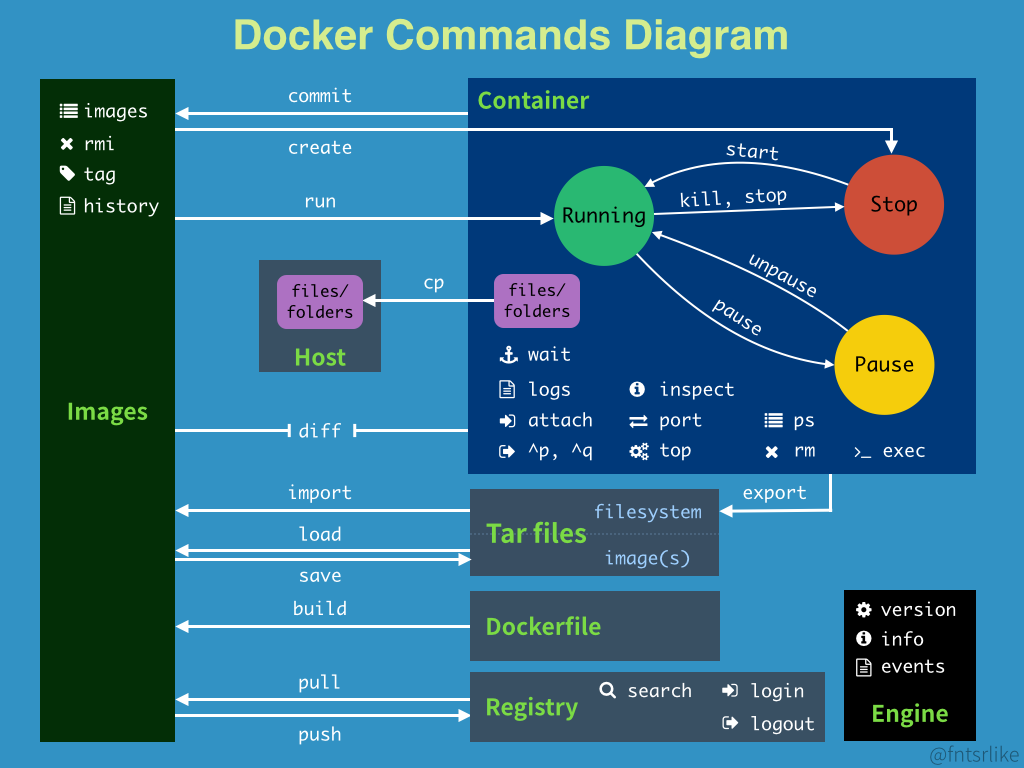
\includegraphics[width=0.9\paperwidth]{Bilder/dockercommand.png}
    \end{textblock*}
\end{frame} 

\begin{frame}
    \frametitle{Weitere Befehle}
    \code{docker images [OPTIONS] [REPOSITORY[:TAG]]}

    \- \ Auflistung von Images\vspace{5pt}

    \code{[OPTIONS]}
    \begin{description}[labelindent=0.5cm, style=unboxed, labelwidth=\widthof{bla}, leftmargin=!]
        \item[\desclabel{-a, -\,-all}] Zeige alle Images (default: intermediate Images versteckt)
        \item[\desclabel{-f, -\,-filter filter}] Filter das Ergebnis
        \item[\desclabel{-\,-format string}] Ausgabe formatieren
    \end{description}\medskip
    \code{docker ps [OPTIONS]}

    \- \ Auflistung von laufenden Containern\vspace{5pt}

    \code{[OPTIONS]}
    \begin{description}[labelindent=0.5cm, style=unboxed, labelwidth=\widthof{bla}, leftmargin=!]
        \item[\desclabel{-a, -\,-all}] Zeige alle Container (auch gestoppte)
        \item[\desclabel{-f, -\,-filter filter}] Filter das Ergebnis
        \item[\desclabel{-\,-format string}] Ausgabe formatieren
        \item[\desclabel{-n, -\,-last int}] Zeige nur die letzten n Container
    \end{description}
\end{frame} 

\begin{frame}[fragile]
    \frametitle{Weitere Befehle}
    \code{docker commit [OPTIONS] CONTAINER [REPOSITORY[:TAG]]}

    \- \ Erstelle ein neues Image aus dem aktuellen Containerzustand\vspace{5pt}

    \code{[OPTIONS]}
    \begin{description}[labelindent=0.5cm, style=unboxed, labelwidth=\widthof{bla}, leftmargin=!]
        \item[\desclabel{-c, -\,-change list}] Verwende Dockerfile instruction zum erstellen
        \item[\desclabel{-m, -\,-message string}] Commit Nachricht
        \item[\desclabel{-p, -\,-pause}] Pausere den Container während des commits (default true)
    \end{description}
    \medskip\medskip
    \code{docker tag SOURCE\_IMAGE[:TAG] TARGET\_IMAGE[:TAG]}\\
    \-  \ Erstelle einen neuen Tag für ein Image \\
    \-  \ \verb|docker image tag 9c62f3337754 ubuntu:v3|\medskip
\end{frame}

\begin{frame}[fragile]
    \frametitle{Weitere Befehle}
    \code{docker cp [OPTIONS] CONTAINER:SRC\_PATH DEST\_PATH|-}

    \- \ Kopiere Dateien zwichen Container und lokalem Speicher\vspace{5pt}

    \code{CONTAINER:SRC\_PATH DEST\_PATH|-} Kopiere von Conatiner zu lokal\\
    \code{SRC\_PATH|- CONTAINER:DEST\_PATH} Kopiere von lokal zu Container\\
    \code{-} Nutze tar archive
    \medskip\medskip
    
    \code{docker import [OPTIONS] file | URL | - [REPOSITORY[:TAG]]}\\
    \-  \ Erstelle ein Image aus einer tar-Datei  \medskip

    \code{docker export [OPTIONS] CONTAINER}\\
    \-  \ Dateisystem eines Containers als tar speichern \medskip

\end{frame}

\begin{frame}[t]
    \frametitle{Andere UseCases}
    \begin{itemize}
        \item \href{https://github.com/OpenDroneMap/WebODM?tab=readme-ov-file}{OpenDrone Map}
        \item Datenbanken in Containern
        \item Kubernetes Cluster
        \item Unternehmen, die wohl Docker nutzen: Airbnb, Spotify, PayPal, Uber, Netflix
        \item \href{https://www.simplilearn.com/docker-use-cases-article}{UseCasees}
    \end{itemize}
\end{frame}

\begin{frame}[t]
    \frametitle{Coole Quellen und so weiter}
    \begin{itemize}
        \item \href{https://www.docker.com/}{https://www.docker.com/}
        \item Offizielle Dokumentation: \href{https://docs.docker.com/get-started/}{https://docs.docker.com/get-started/}
        \item \href{https://www.heise.de/news/Wie-man-Docker-auf-dem-Raspberry-Pi-in-15-Minuten-einrichtet-7524692.html}{Wie man Docker auf Rasberry Pi einrichtet}
    \end{itemize} 
    \begin{block}{Weitere Themen für Lightning Talks und Full Talks}
        \begin{itemize}
            \item Docker Networks
            \item Docker Compose (ausführlicher)
            \item Kubernetes
        \end{itemize}
        
    \end{block}
\end{frame}

\end{document}